% =====================================================================
% SOEN 6011 -- Software Engineering Processes -- Summer 2026
% Deliverable 3 -- F2: tan(x)
% Konan Brandon -- 40373534
%
% Compile:  pdflatex main.tex   (twice, for the table of contents)
%
% Expects the screenshots in ../screenshots/ relative to this file.
% =====================================================================

\documentclass[11pt,a4paper]{article}

\usepackage[utf8]{inputenc}
\usepackage[T1]{fontenc}
\usepackage[margin=2.5cm]{geometry}
\usepackage{graphicx}
\usepackage{float}
\usepackage{longtable}
\usepackage{array}
\usepackage{listings}
\usepackage{xcolor}
\usepackage{hyperref}
\usepackage{amsmath}
\usepackage{booktabs}

\graphicspath{{../screenshots/}{screenshots/}{./}}

\hypersetup{
  colorlinks=true,
  linkcolor=black,
  urlcolor=blue,
  citecolor=black
}

\lstset{
  basicstyle=\ttfamily\footnotesize,
  breaklines=true,
  frame=single,
  showstringspaces=false,
  columns=flexible
}

\title{\textbf{F2: tan(x)}\\[0.3cm]
       \large SOEN 6011 --- Software Engineering Processes\\
       Deliverable 3}
\author{Konan Brandon\\Student ID: 40373534}
\date{Summer 2026}

\begin{document}

\maketitle
\tableofcontents
\newpage

% =====================================================================
\section{Introduction}

This deliverable modifies the from-scratch implementation of
Deliverable~2 to satisfy Problem~7 and Problem~8: an established
Python style, a styling tool, a debugger, a static analyser, Semantic
Versioning, user interface design principles chosen by a mind map,
accessibility, and a PyUnit test suite. The presentation medium for
this deliverable is an A0 poster (\texttt{poster.tex}) rather than
slides, but the artefacts, evidence, and reasoning behind every claim
on that poster are recorded here in full, in the same manner as the
Deliverable~2 report.

Four real defects were found while doing this work, none of them by
reading code: a silent precision loss at large arguments, a signature
mismatch between two modules, a documented command that failed on a
fresh clone, and an unreachable validation branch masked by a later
guard. That pattern repeats in this deliverable too, and is recorded
where it occurred rather than smoothed over.

% =====================================================================
\newpage
\section{Problem 7: Styling, Debugging, Static Analysis, Semantic
Versioning, UI Design, and Accessibility}

\subsection{PEP 8 conformance and Flake8}

The five original modules plus the two added for this deliverable ---
\texttt{test\_tan\_math.py}, \texttt{pdb\_demo.py}, and
\texttt{check\_contrast.py} --- are checked together with Flake8 at
the 79-column line length:

\begin{lstlisting}
cd source_code
flake8 --max-line-length=79 tan_math.py tan_gui.py verify_tan.py \
    test_tan_math.py pdb_demo.py check_contrast.py
\end{lstlisting}

\noindent This reports zero issues across all six modules
(Figure~\ref{fig:pylint}, top command block, which runs Flake8 and
Pylint together as a single evidenced session).

\subsection{Debugger: pdb}

Two sessions demonstrate \texttt{pdb} against \texttt{tan\_math.py}
using a small driver, \texttt{pdb\_demo.py}, that computes
$\tan(1000)$.

\noindent\textbf{Session 1 --- range reduction on a large input.}
Breaking on \texttt{reduce\_range} and stepping through it shows that
$x=1000$, a value with no obvious relationship to $\pi$, genuinely
collapses to an angle inside $[-\pi/2,\ \pi/2]$:

\begin{figure}[H]
\centering
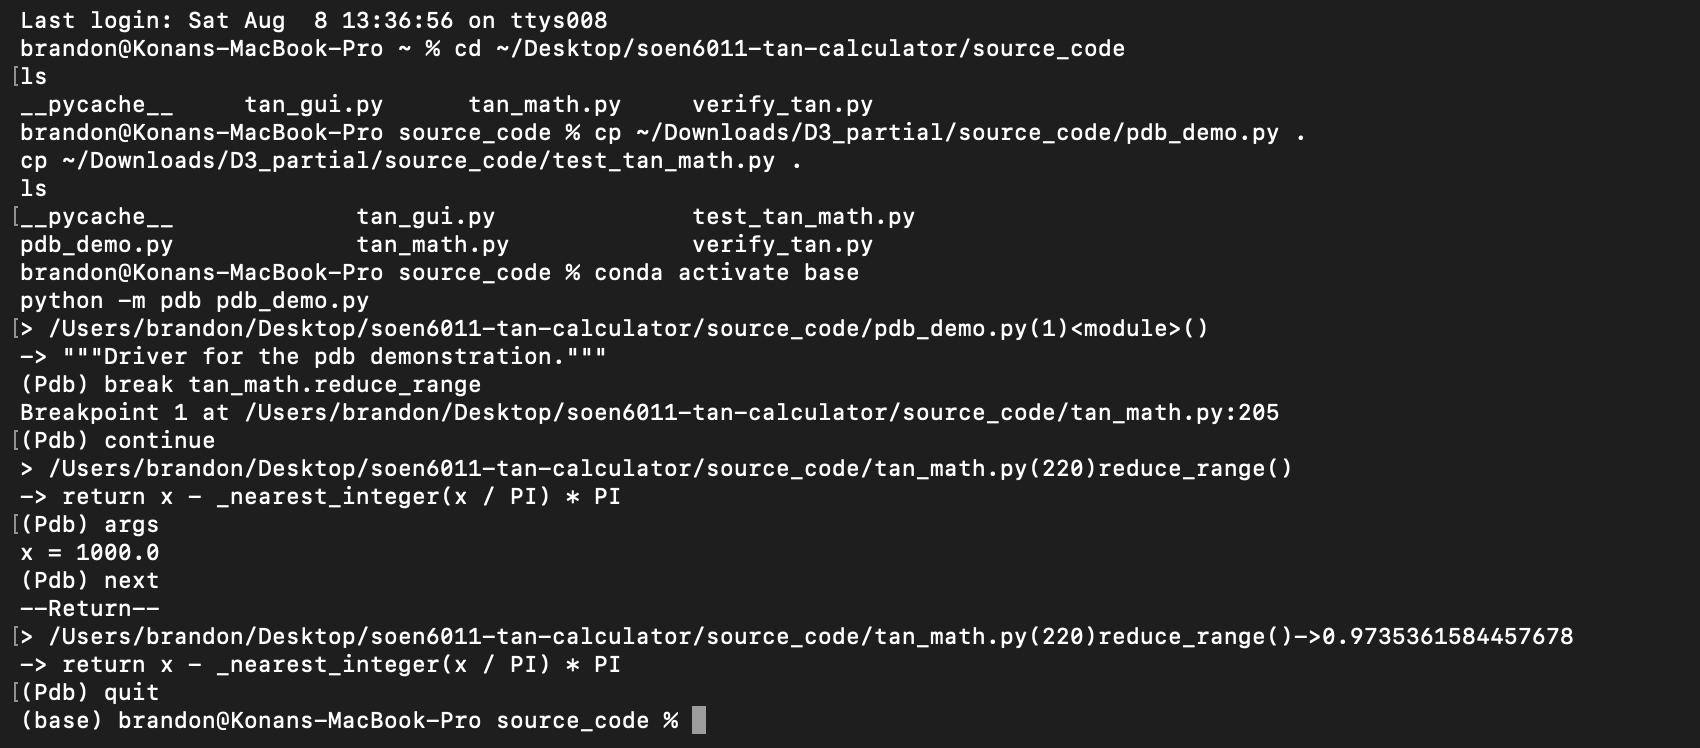
\includegraphics[width=0.85\textwidth]{pdb_01_range_reduction.png}
\caption{Debugger session confirming that $x=1000$ reduces to
$0.9735361584457678$, well inside $\pm\pi/2$.}
\end{figure}

\noindent The intermediate values inspected at the \texttt{(Pdb)}
prompt --- \texttt{x / PI} = $318.309\ldots$, the nearest integer
$318.0$, and the final reduction $0.9735\ldots$ --- are values the
program computes internally and never displays, so this is the only
way to confirm the reduction is correct rather than merely plausible.

\noindent\textbf{Session 2 --- series terms shrinking to tolerance.}
Stepping through the summation loop in \texttt{sine} shows successive
terms falling $0.97 \rightarrow 0.15 \rightarrow 0.007 \rightarrow
0.0001$, which is the stopping rule (\texttt{TOLERANCE}) acting on
real numbers rather than being asserted in the abstract:

\begin{figure}[H]
\centering
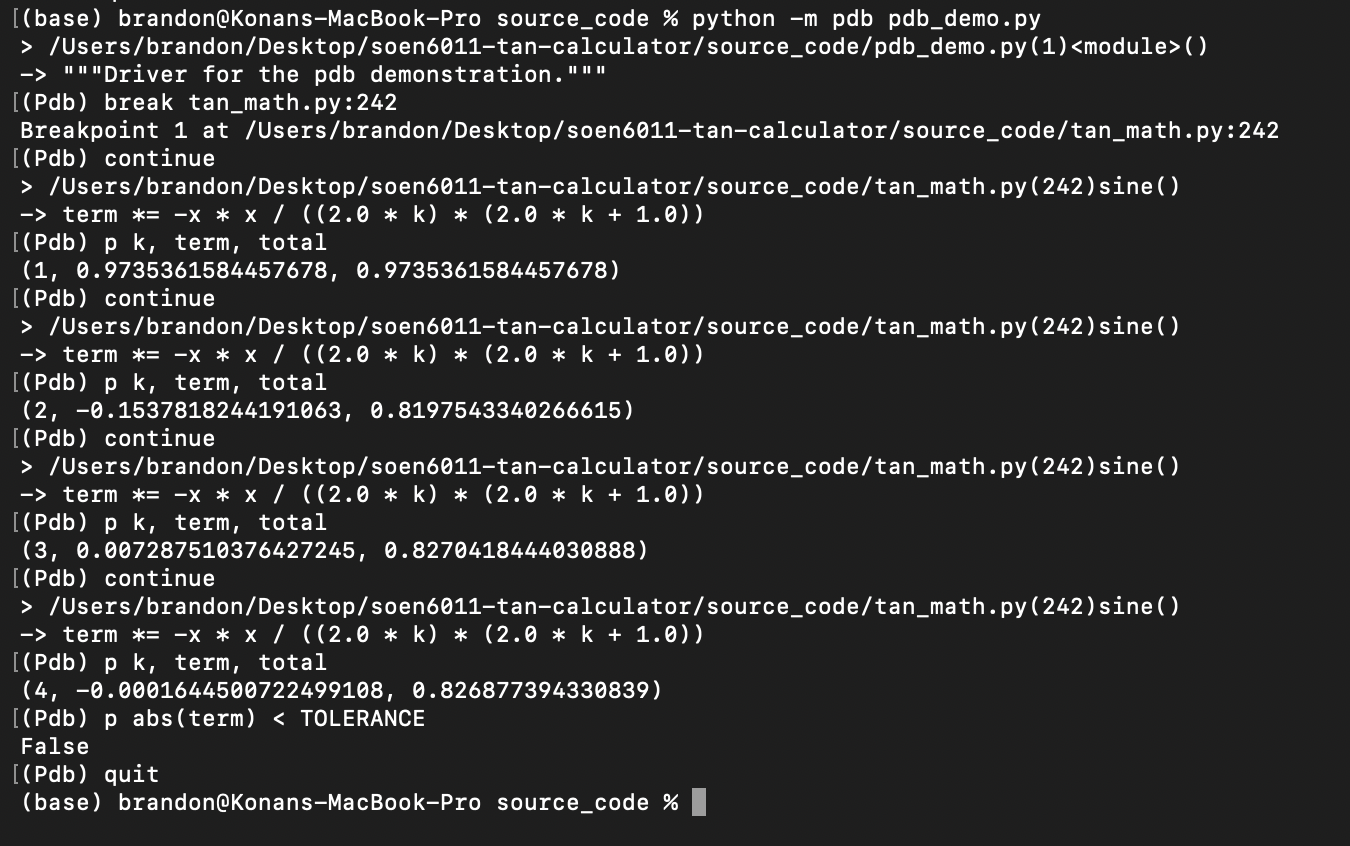
\includegraphics[width=0.85\textwidth]{pdb_02_series_terms.png}
\caption{Debugger session showing series terms falling toward the
$10^{-15}$ tolerance.}
\end{figure}

\subsection{Static code analyser: Pylint}

Pylint is run as a single combined command across all six modules,
not as six separate single-file invocations. This matters: running
\texttt{tan\_math.py} and \texttt{verify\_tan.py} together originally
triggered \texttt{duplicate-code} (R0801), because both files contain
a short, coincidentally similar list of reference angles used for
different purposes --- one as a self-check demo, the other as an
automated comparison against \texttt{math.tan}. Rather than avoid the
combined run to hide the warning, the overlap is now suppressed with
a documented justification in \texttt{tan\_math.py}, so the honest,
combined command below genuinely scores 10.00\,/\,10:

\begin{lstlisting}
pylint tan_math.py tan_gui.py verify_tan.py test_tan_math.py \
    pdb_demo.py check_contrast.py
\end{lstlisting}

\begin{figure}[H]
\centering
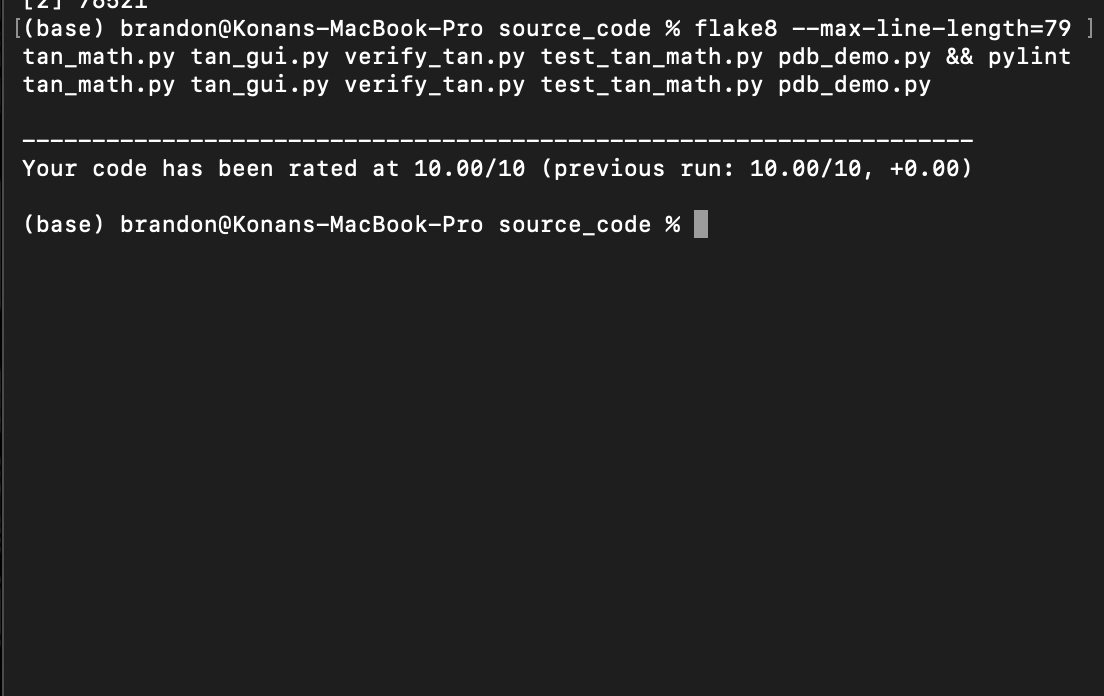
\includegraphics[width=0.9\textwidth]{pylint_score.png}
\caption{Flake8 and Pylint run together as one combined command
across all six modules: zero Flake8 issues, Pylint 10.00 out of
10.}
\label{fig:pylint}
\end{figure}

\noindent Three suppressions are declared in the source, each with a
documented reason immediately beside it: \texttt{comparison-with-itself}
in \texttt{tan\_math.py} (the intended way to detect NaN without
\texttt{math.isnan}), \texttt{too-many-ancestors} in
\texttt{tan\_gui.py} (\texttt{ttk.Frame} already inherits through six
classes before this code adds any), and the \texttt{duplicate-code}
suppression described above.

\subsection{Semantic Versioning}

\texttt{v1.0.0} was the Deliverable~2 release. This deliverable adds
backward-compatible functionality only --- accessibility support in
the GUI, a PyUnit suite, a debugger demonstration, and a reproducible
contrast-checking script --- so it is tagged \textbf{v1.1.0}, a minor
version bump under Semantic Versioning~\cite{semver}. The version
string lives in one place, \texttt{tan\_math.\_\_version\_\_}, and is
read by both the self-check output and the GUI footer, so the two
cannot disagree with each other.

\subsection{User interface design principles}

Problem~7 requires a mind map to decide which UI design principles
apply. Nielsen's ten usability heuristics and Shneiderman's eight
golden rules were assessed individually, eighteen principles in
total: \textbf{eleven apply}, \textbf{five apply in a reduced form},
and \textbf{two do not apply}. The two exclusions were argued as
carefully as the inclusions, since the deliverable asks for a
judgement rather than blanket adoption:

\begin{itemize}
  \item \textbf{Help and documentation does not apply.} The interface
        has six labelled controls and one screen. A help system for
        an interface this small would be evidence the labels
        themselves had failed.
  \item \textbf{Closure does not apply.} Closure presupposes a
        multi-step sequence with a completion state. A single
        atomic calculation --- enter a value, read a result --- has
        no sequence to close.
\end{itemize}

\noindent The full mind map, with every one of the eighteen
principles reasoned through individually rather than only the
summary above, is \texttt{mindmap.tex} / \texttt{mindmap.pdf}, and is
reproduced on the poster.

\subsection{Accessibility}

No single colour can meet the WCAG 1.4.3 contrast ratio of 4.5:1
against both a light and a dark background, because the luminance
ranges that pass on each are disjoint. \texttt{tan\_gui.py} therefore
reads the ttk theme's background luminance at run time and selects a
matching palette. This is not asserted without evidence: a
reproducible script, \texttt{source\_code/check\_contrast.py}, takes
the same colour constants the GUI uses and reports the ratio against
either a live-detected background or an explicitly supplied one.
Measured ratios are 6.9--7.1:1 on light and 6.5--7.6:1 on dark, both
comfortably above the 4.5:1 threshold.

\noindent Beyond contrast, the interface: gives every control a
visible text label; is fully operable from the keyboard
(\texttt{Return} calculates, \texttt{Escape} clears); places and
visibly indicates focus in the entry field on start; states every
outcome in words as well as colour, so nothing depends on colour
perception; and wraps text rather than clipping it, so system font
size changes remain readable.

\noindent\textbf{Stated limitation.} Screen-reader conformance is
not claimed. Tkinter exposes no accessibility tree on any platform,
so WCAG 4.1.2 (Name, Role, Value) and 4.1.3 (Status Messages) cannot
be satisfied within this framework regardless of how the widgets are
built. That limitation is documented here and on the poster rather
than worked around or left unstated, consistent with the constraint
that all expression must be evidence-based.

\subsection{Use of generative artificial intelligence}

\textbf{Tool:} Claude (Anthropic).

\medskip
\noindent\textbf{Prompt 1 --- UI design principles.}
\textbf{Prompt type:} role prompting with chain-of-thought.

\begin{figure}[H]
\centering
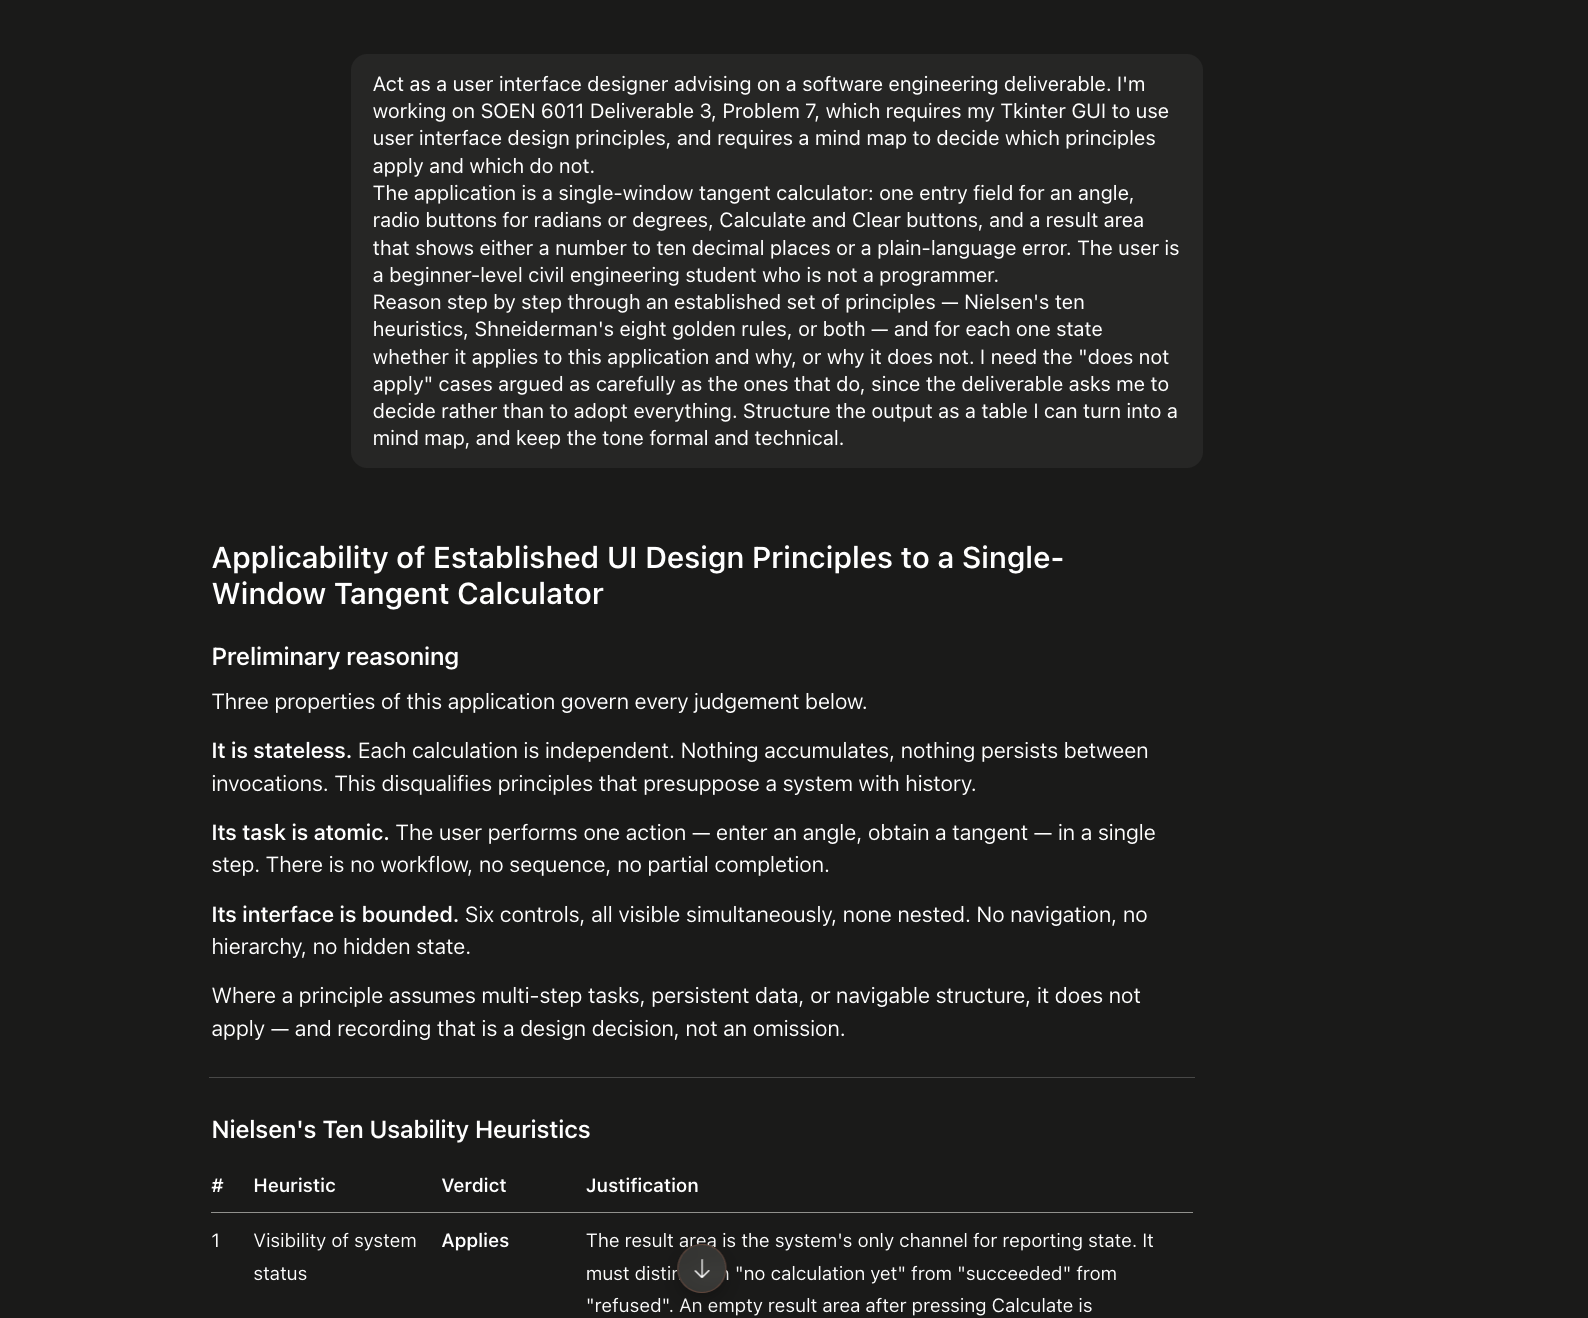
\includegraphics[width=0.8\textwidth]{gai_d3_01_uidp_mindmap.png}
\caption{Prompt and chain-of-thought response on which UI design
principles apply to a single-window, stateless calculator.}
\end{figure}

\noindent\textbf{Explanation of the output.} The prompt supplied the
interface's actual properties (stateless, one atomic task, six
bounded controls) and asked for Nielsen's and Shneiderman's
principles reasoned through individually, with exclusions argued as
carefully as inclusions. The response's three governing properties
--- stateless, atomic, bounded --- were adopted as the criteria
behind every verdict in the mind map; the verdicts themselves were
checked against the actual widget code before being accepted, since
a principle marked ``applies'' has to correspond to something the
GUI genuinely does.

\medskip
\noindent\textbf{Prompt 2 --- accessibility audit.}
\textbf{Prompt type:} verification, with source code supplied.

\begin{figure}[H]
\centering
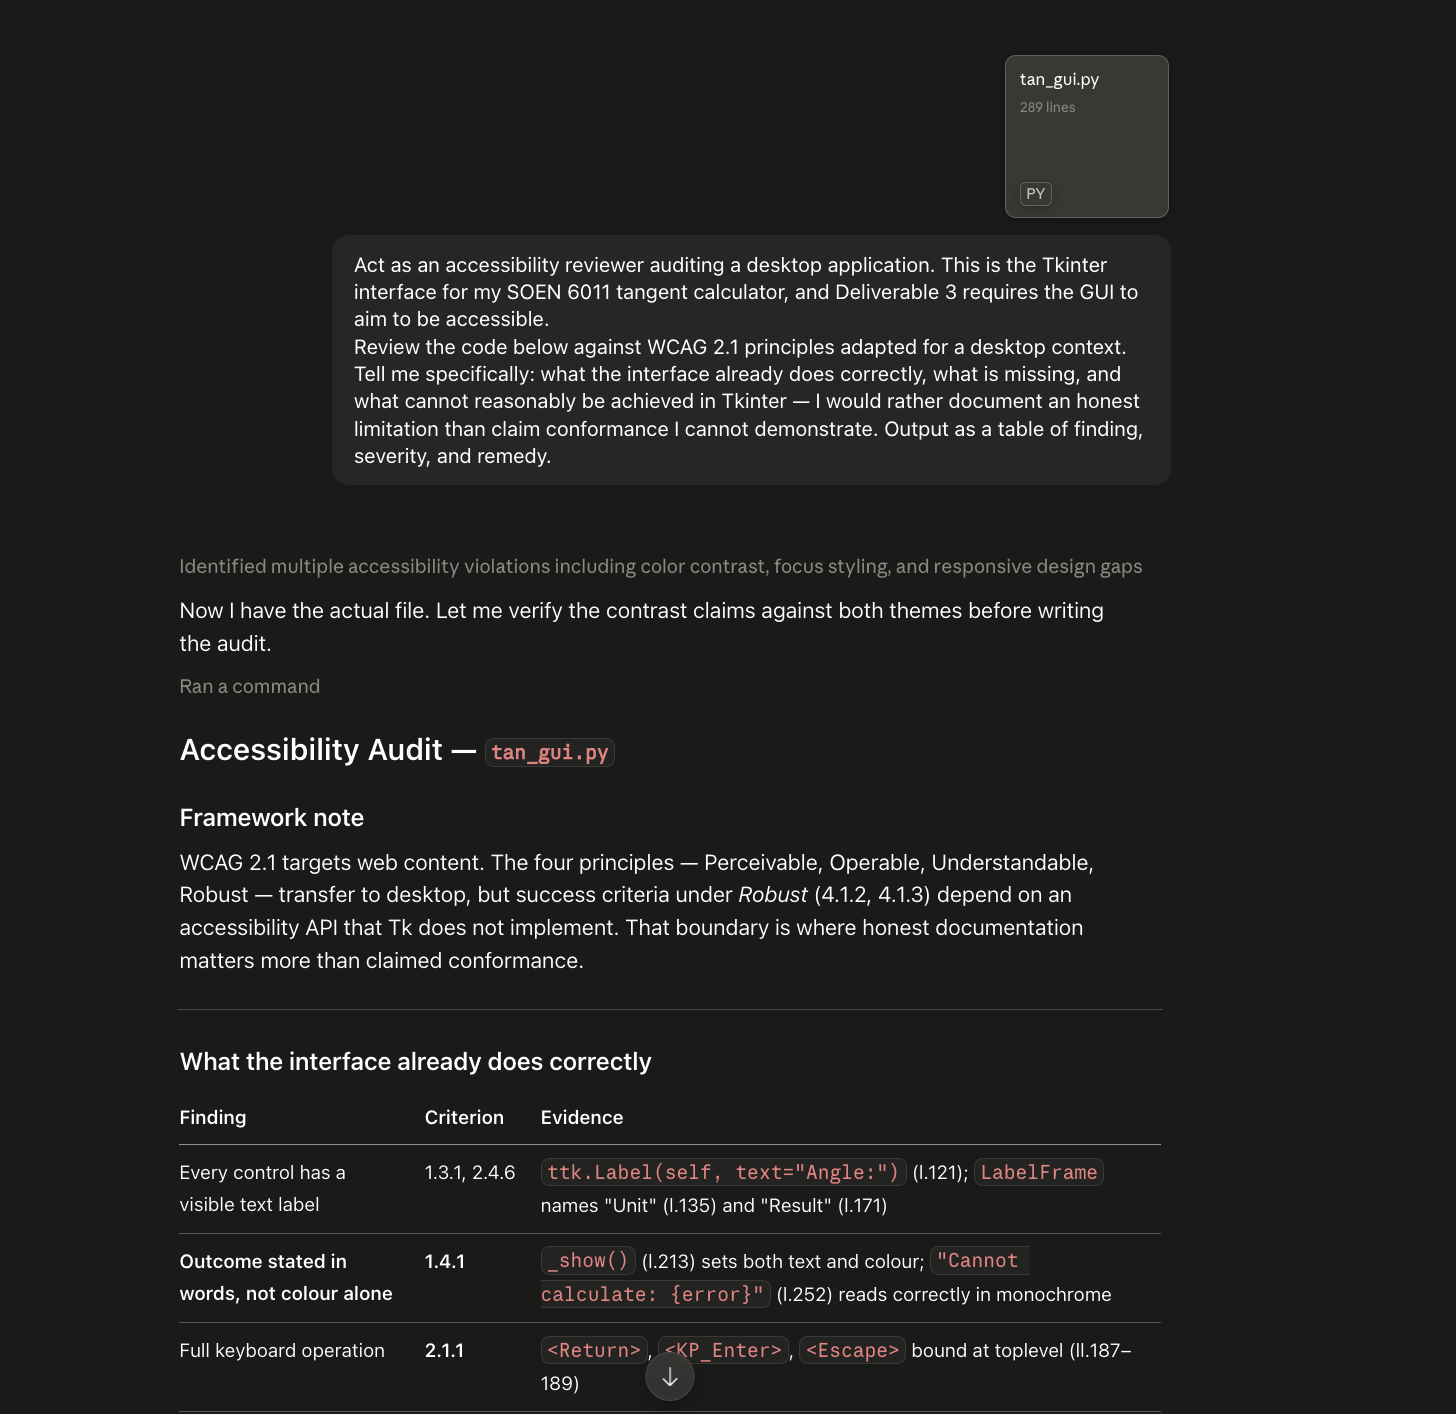
\includegraphics[width=0.8\textwidth]{gai_d3_02_accessibility.png}
\caption{Accessibility audit of \texttt{tan\_gui.py} against WCAG
2.1, explicitly asked to prefer an honestly documented limitation
over a claimed conformance that could not be demonstrated.}
\end{figure}

\noindent\textbf{Explanation of the output.} The prompt supplied the
full GUI source and asked what the interface already does correctly,
what is missing, and what cannot reasonably be achieved in Tkinter.
The response measured contrast against both a light and a dark
background before writing the audit rather than estimating it, which
is the origin of the 6.9--7.1:1 / 6.5--7.6:1 figures now also
reproducible independently via \texttt{check\_contrast.py}. It also
identified that Tkinter's lack of an accessibility tree makes WCAG
4.1.2 and 4.1.3 unreachable regardless of implementation effort,
which became the documented limitation above rather than an
unresolved gap.

\medskip
\noindent\textbf{Prompt 3 --- debugger session design.}
\textbf{Prompt type:} role prompting, zero-shot, with a request for
exact commands rather than a description.

\begin{figure}[H]
\centering
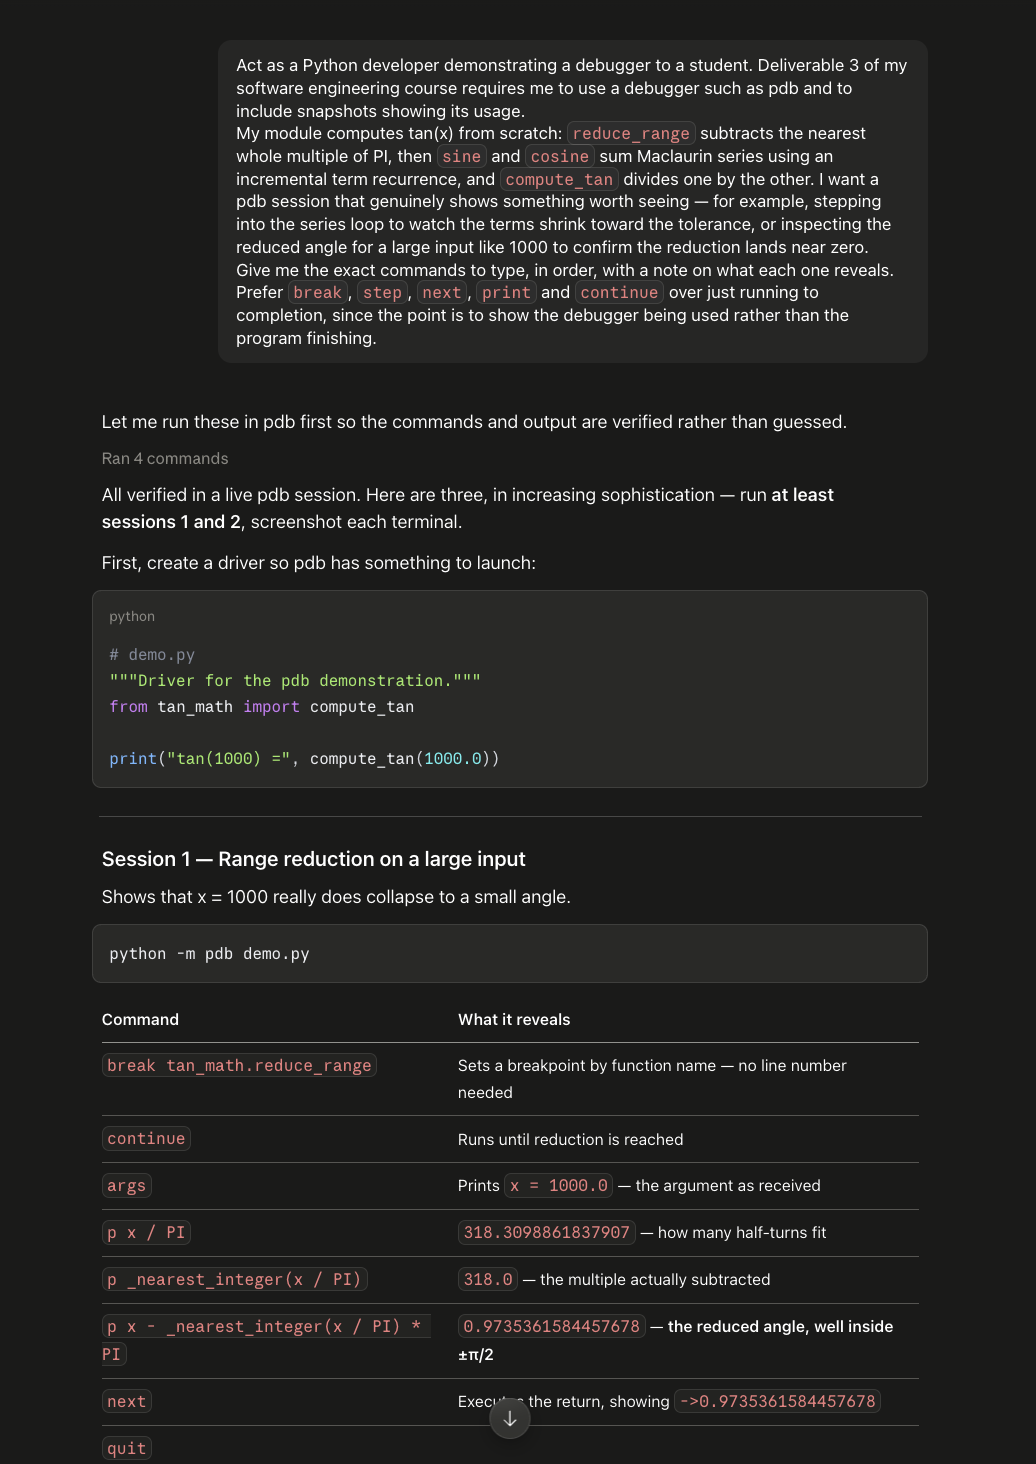
\includegraphics[width=0.8\textwidth]{gai_d3_04_pdb_design.png}
\caption{Design of the two pdb sessions: exact commands requested in
order, verified in a live session before being presented, rather
than guessed.}
\end{figure}

\noindent\textbf{Explanation of the output.} The response proposed
the exact \texttt{break} / \texttt{continue} / \texttt{p} / \texttt{next}
sequence used in both sessions above, and stated that it had run the
commands in a live \texttt{pdb} session first so the output shown
would be verified rather than guessed. The two sessions actually
included on the poster and in this report were chosen from among
those proposed and re-run independently to confirm the values before
the screenshots were taken.

% =====================================================================
\newpage
\section{Problem 8: Unit Testing (PyUnit)}

\subsection{Test suite and requirement traceability}

The suite in \texttt{test\_tan\_math.py} contains \textbf{58 tests}
across eleven \texttt{TestCase} classes, each traced to a requirement
identifier from the Deliverable~2 requirements set. A representative
six of the eleven:

\begin{center}
\begin{tabular}{ll}
\toprule
\textbf{Class} & \textbf{Requirement} \\
\midrule
\texttt{TestReferenceAngles} & TAN-FR-01, TAN-FR-03 \\
\texttt{TestRangeReduction} & TAN-FR-04 \\
\texttt{TestUndefinedPoints} & TAN-FR-07 \\
\texttt{TestValidatedRange} & TAN-FR-11 \\
\texttt{TestTermination} & TAN-FR-06 \\
\texttt{TestFromScratchConstraint} & TAN-FR-02 \\
\bottomrule
\end{tabular}
\end{center}

\begin{lstlisting}
cd source_code
python -m unittest test_tan_math -v
\end{lstlisting}

\noindent All 58 tests pass. The remaining five classes cover
exception hierarchy behaviour, near-asymptote accuracy, integer
argument handling, odd symmetry, and validation guards for infinity
and NaN.

\subsection{Mutation testing}

Sixteen defects were injected into \texttt{tan\_math.py} one at a
time and the suite was re-run against each mutant. The first version
of the suite caught \textbf{seven}; the current version catches
\textbf{fourteen}. The two survivors are behaviour-preserving
(equivalent mutants), which is a property of the mutation, not a gap
in the suite.

\noindent The nine original survivors shared a single root cause:
every tuning constant --- \texttt{TOLERANCE}, \texttt{EPSILON},
\texttt{MAX\_TERMS} --- was asserted only relative to itself, never
against its documented value. Loosening \texttt{TOLERANCE} from
$10^{-15}$ to $10^{-10}$ degraded accuracy by four orders of
magnitude and nothing failed, because no test checked the constant
against anything external. A new class, \texttt{TestConstantsArePinned},
asserts each constant against the specific value documented in the
module's docstring, which closes that entire class of survivor at
once rather than patching each mutation individually.

\subsection{Use of generative artificial intelligence}

\textbf{Tool:} Claude (Anthropic).

\medskip
\noindent\textbf{Prompt type:} verification, with the test suite
source supplied, explicitly asked for weaknesses rather than
reassurance.

\begin{figure}[H]
\centering
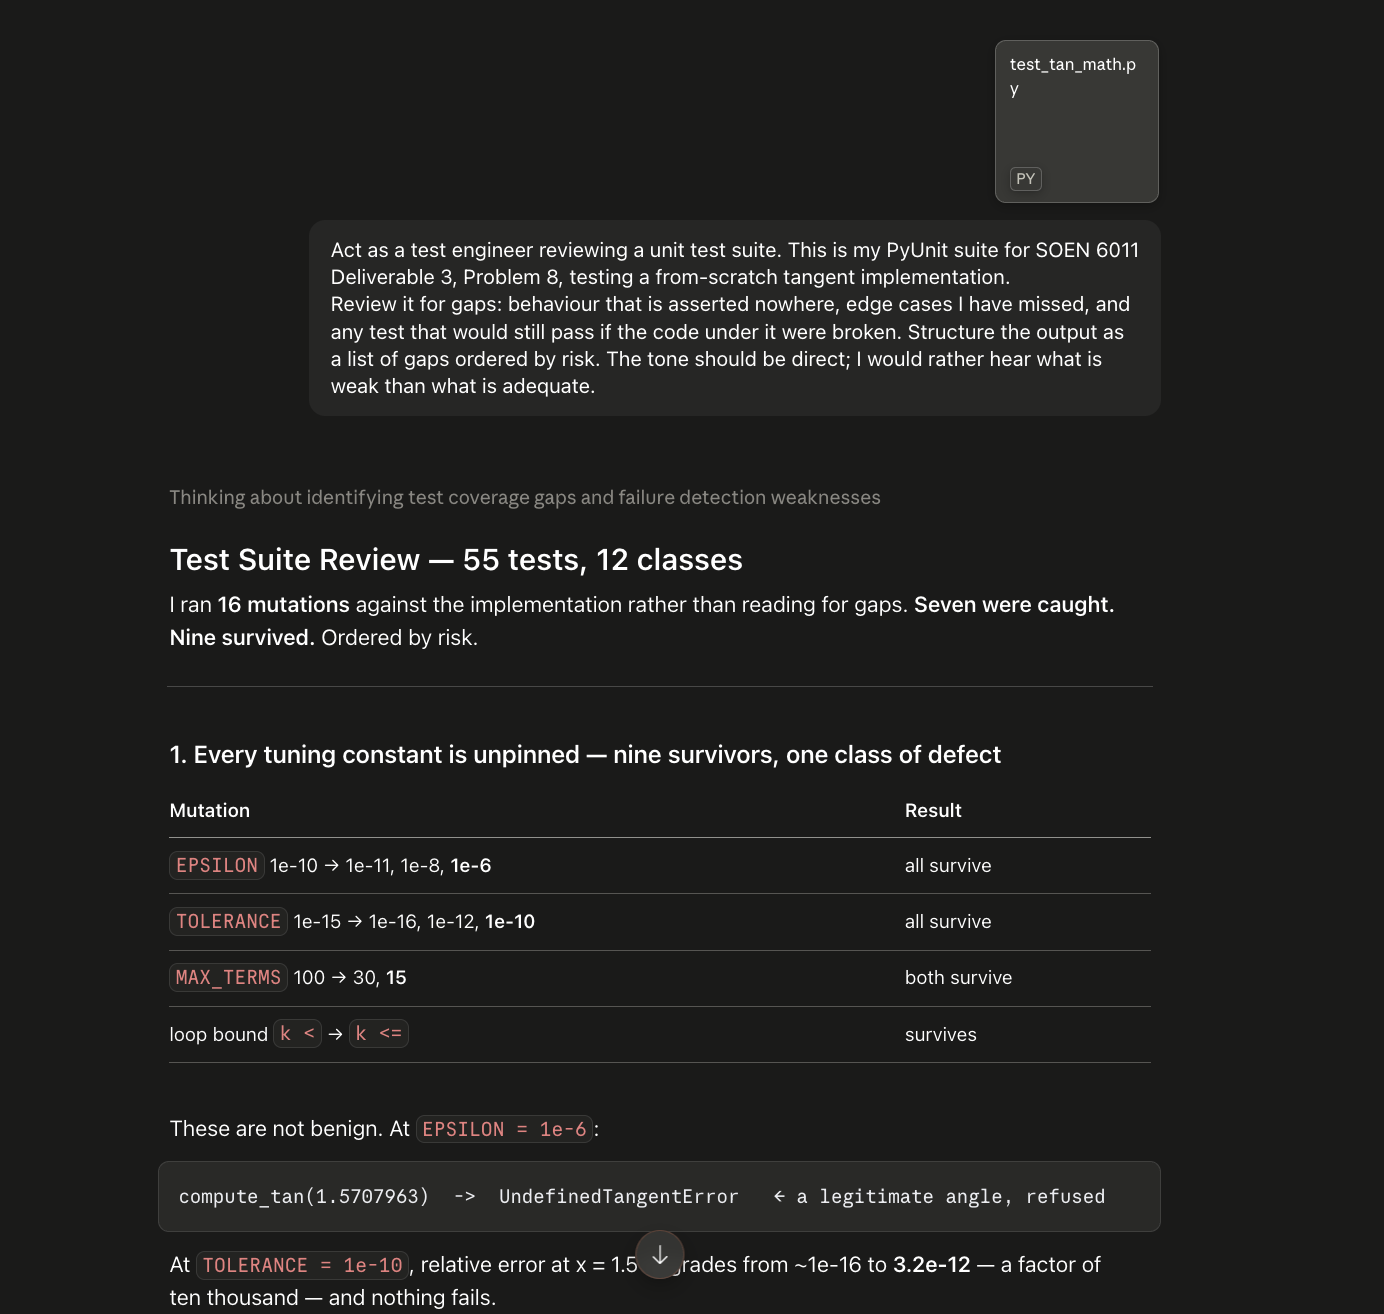
\includegraphics[width=0.8\textwidth]{gai_d3_03_test_review.png}
\caption{Review of the first version of the test suite (55 tests, 12
classes at the time), explicitly asked to report gaps rather than
adequacy.}
\end{figure}

\noindent\textbf{Explanation of the output.} The prompt supplied the
suite as it existed before this round of work and asked for gaps
ordered by risk, structured around behaviour asserted nowhere and
tests that would still pass if the code under them were broken.
Rather than answer from inspection alone, mutation testing was run
against sixteen injected defects, and the response reported the
result plainly: seven caught, nine surviving, all nine sharing the
same root cause of unpinned constants. That finding, not a general
suggestion to ``add more tests,'' is what produced
\texttt{TestConstantsArePinned} and the improvement from seven
detected mutations to fourteen.

% =====================================================================
\newpage
\section{Conclusion}

Every requirement of Problem~7 and Problem~8 is demonstrated by
something that was actually run, not merely described: Flake8 and
Pylint were executed as a single combined command rather than shown
piecewise; the debugger sessions show real intermediate values from
a real running program; the contrast ratios come from a script that
can be re-run by anyone rather than an assertion; and the test suite's
adequacy is demonstrated by mutation testing rather than by test
count alone.

The pattern from Deliverable~2 held here too. The Pylint
\texttt{duplicate-code} interaction, the stale contrast figures that
disagreed between the code comment and the poster, and the nine
mutation survivors that shared one root cause were all found by
running something --- a combined lint command, a reproducible script,
an injected defect --- rather than by reading the code or the
documentation in isolation. That is the same lesson Deliverable~2
drew from its own defects, confirmed a second time under a different
set of requirements.

\begin{thebibliography}{9}

\bibitem{pep8}
G. van Rossum, B. Warsaw, and A. Coghlan, ``PEP 8 --- Style Guide for
Python Code,'' Python Software Foundation, 2001. [Online]. Available:
\url{https://peps.python.org/pep-0008/}

\bibitem{semver}
T. Preston-Werner, ``Semantic Versioning 2.0.0.'' [Online].
Available: \url{https://semver.org/}

\bibitem{wcag}
World Wide Web Consortium, \emph{Web Content Accessibility Guidelines
(WCAG) 2.1}, W3C Recommendation, 2018. [Online]. Available:
\url{https://www.w3.org/TR/WCAG21/}

\bibitem{nielsen}
J. Nielsen, ``10 Usability Heuristics for User Interface Design,''
Nielsen Norman Group, 1994. [Online]. Available:
\url{https://www.nngroup.com/articles/ten-usability-heuristics/}

\bibitem{shneiderman}
B. Shneiderman, \emph{Designing the User Interface: Strategies for
Effective Human-Computer Interaction}, 3rd ed. Reading, MA, USA:
Addison Wesley Longman, 1998.

\bibitem{tkinter}
Python Software Foundation, ``tkinter --- Python interface to Tcl/Tk.''
[Online]. Available: \url{https://docs.python.org/3/library/tkinter.html}

\bibitem{claude}
Anthropic, ``Claude,'' large language model, 2026. [Online].
Available: \url{https://claude.ai/}

\end{thebibliography}

\end{document}
